
\section{Sensor Setup}

\subsection{Light Curtain Basics}

\begin{figure}[h]
   \centering
   \begin{minipage}{0.5\textwidth}
       \centering
       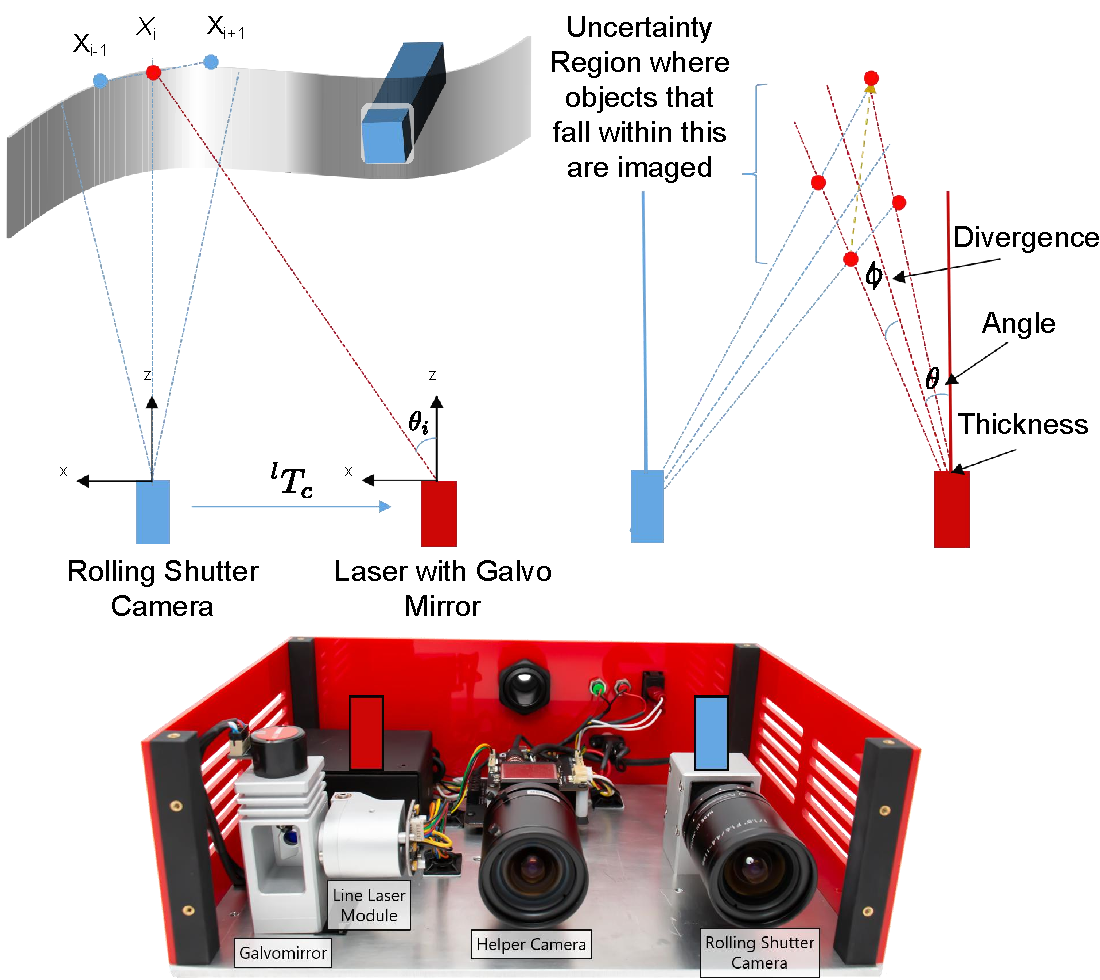
\includegraphics[width=1.0\textwidth]{figures/LC.pdf} % first figure itself
   \end{minipage}\hfill
   % \begin{minipage}{0.3\textwidth}
   %     \centering
   %     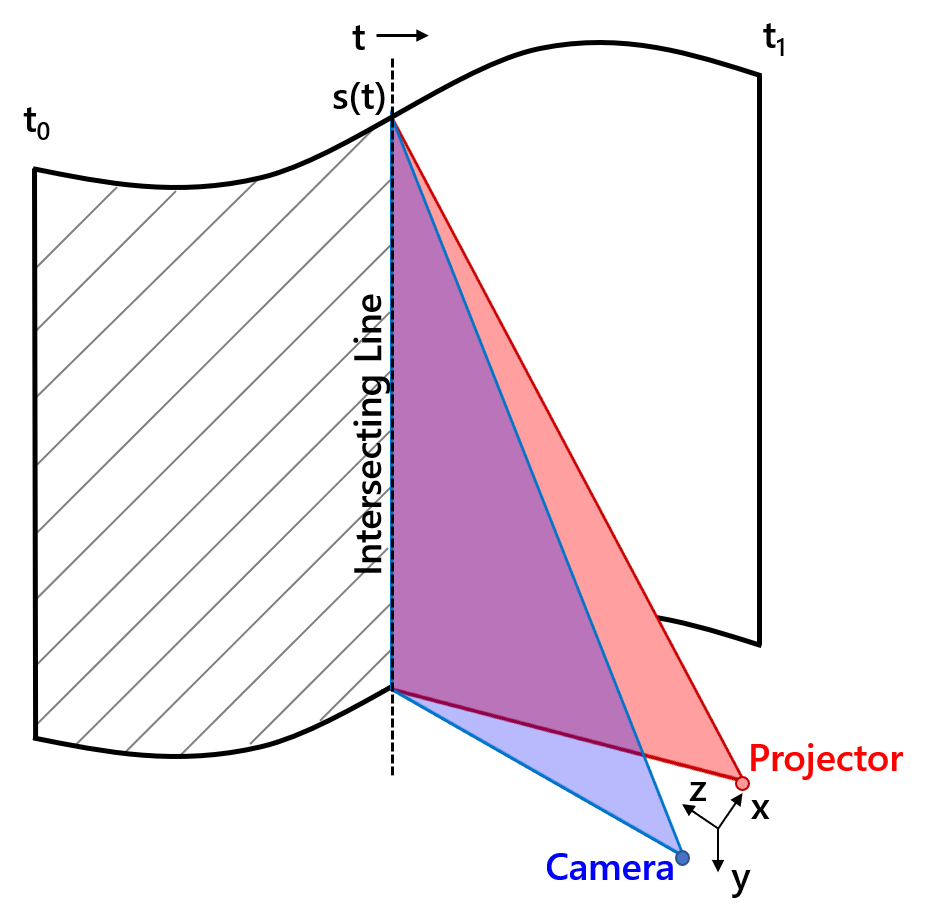
\includegraphics[width=0.9\textwidth]{light_curtain_iso.png} % second figure itself
   % \end{minipage}
   \centering
   \caption{\textbf{Above:} The user provides a top-down 2D curve, which results in a 3D ruled surface being sensed (a form of gated depth imaging). Surfaces that fall within the \textit{thickness} of the curtain, shows up with higher intensity. \textbf{Below:}  The Programmable Light Curtain device (Image taken from \cite{bartels2019Agile}), consisting of a steerable laser, galvo and NIR camera.}
\end{figure}

The Light Curtain consists of a rolling shutter NIR camera flipped vertically (that images a plane in the world per pixel row), a Line Laser module and a Galvomirror (that generates a plane of light in the world depending on the angle). These planes have some divergence, so their intersection results in a volume in space (bounded by purple points) with some \textit{thickness}, where any objects that intersect it show up with higher intensity returns. Sweeping this Laser across, results in a 3D Ruled surface, analogous to gated depth imaging.

\subsection{Simulator}

\begin{figure}[h]
   \centering
   \begin{minipage}{0.4\textwidth}
       \centering
       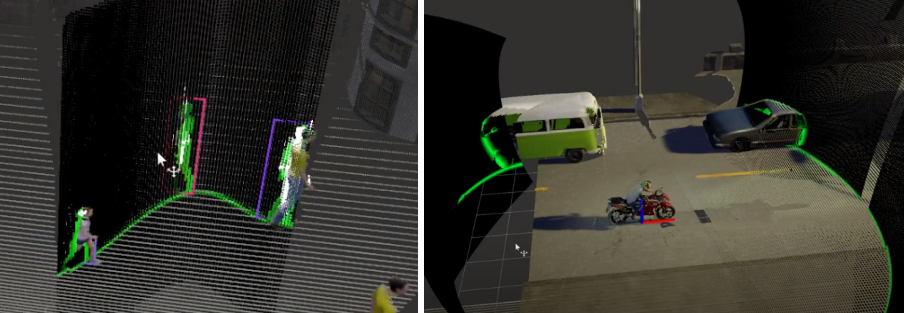
\includegraphics[width=1.0\textwidth]{figures/sim.png}
   \end{minipage}\hfill
   \centering
   \caption{Light Curtain Simulator in CARLA environment}
\end{figure}
%\vspace{-.1in}
We also designed and open sourced a light curtain simulator \cite{raaj2019} to test and evaluate our algorithms, allowing for the Light Curtain paramters such as NIR instrinsics, Laser/NIR extrinsincs, Galvomirror speed etc. to be controlled.

\subsection{Sensor Array}

\begin{figure}[h]
   \centering
   \begin{minipage}{0.5\textwidth}
       \centering
       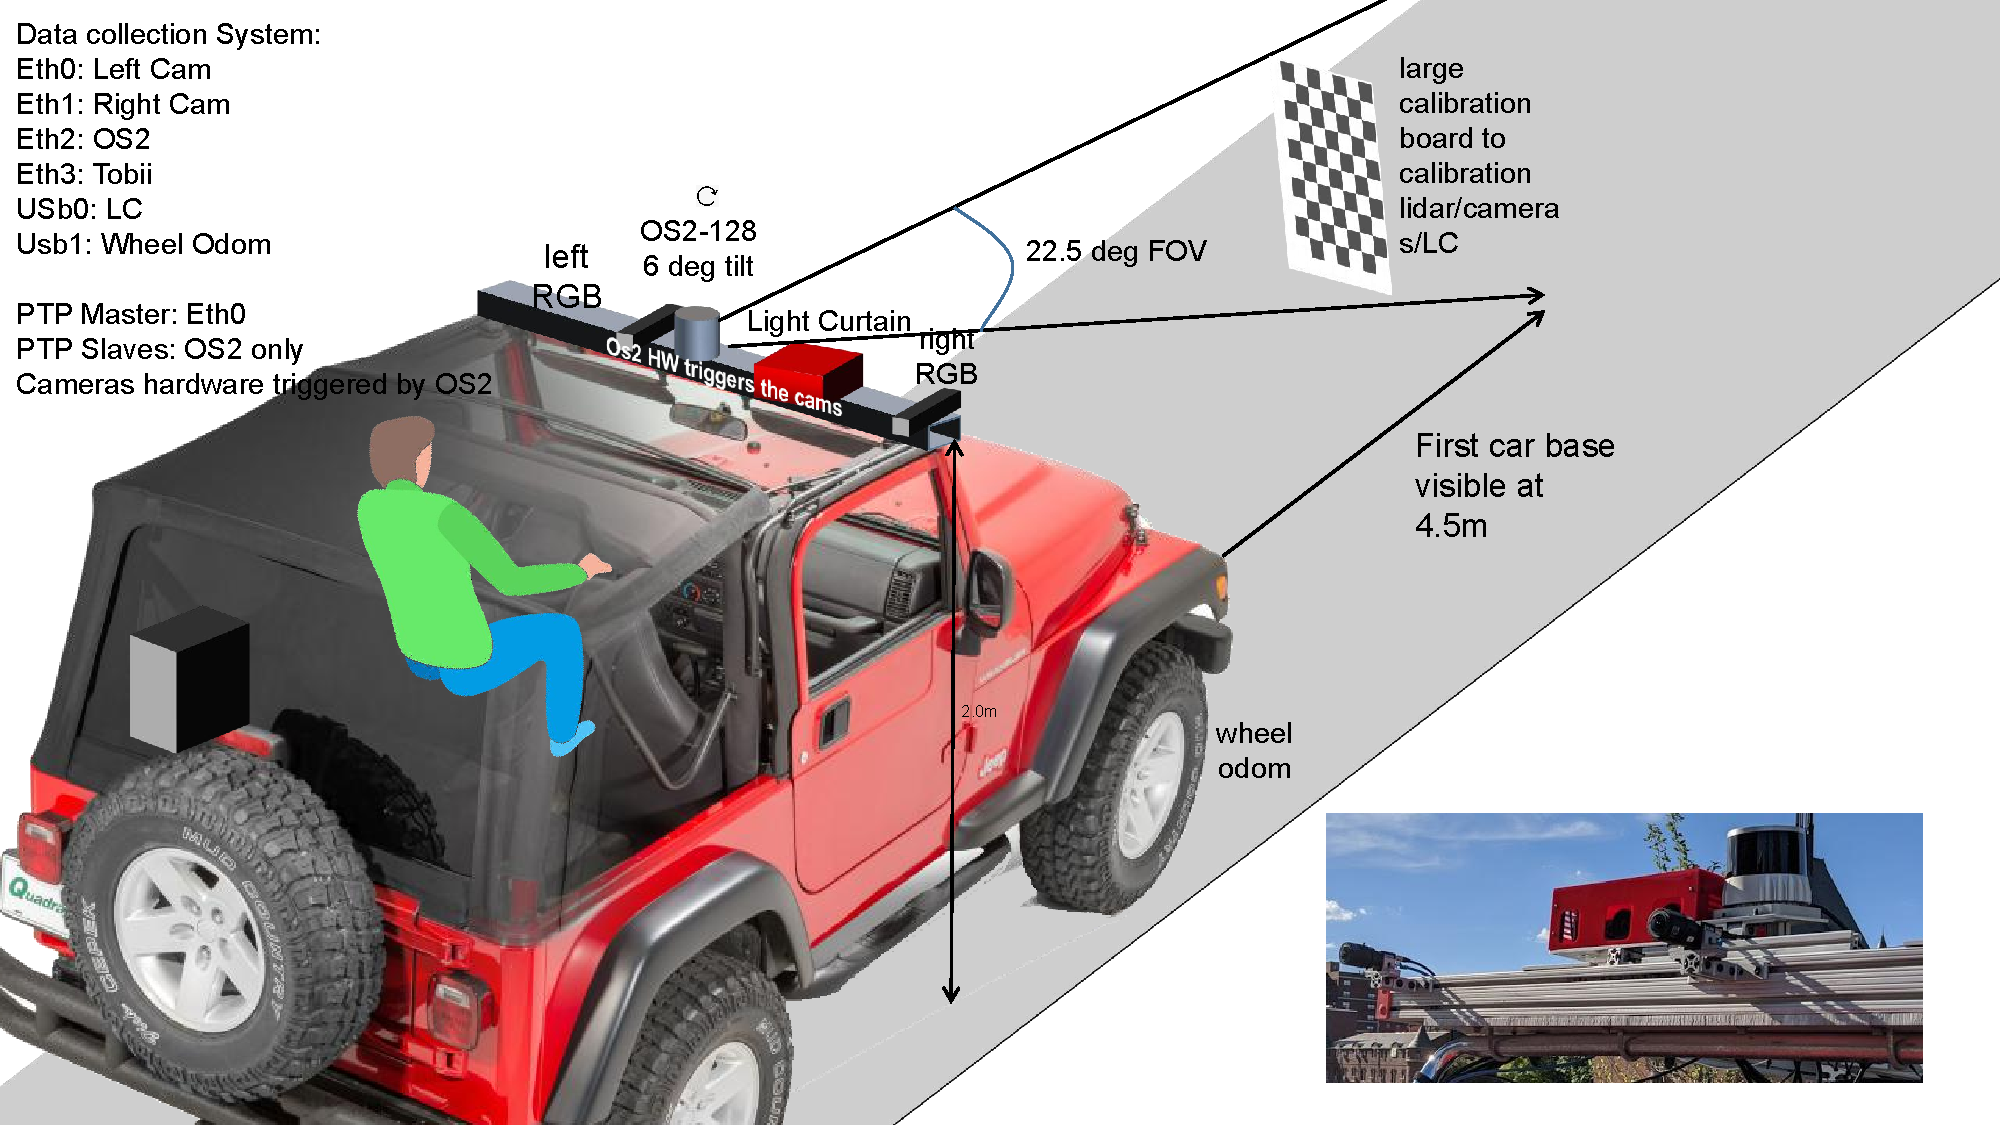
\includegraphics[width=1.0\textwidth]{figures/array.pdf}
   \end{minipage}\hfill
   \centering
   \caption{Sensor Array consisting of a Stereo camera pair, the Light Curtain device and a 128 Beam Lidar}
\end{figure}

Our sensor array consists of a Stereo Camera Pair with a baseline of 0.7m, the Light Curtain device located close to the main/left camera to minimize depth/volume transformation parallax artifacts, and an Ouster OS2-128 Lidar for algorithm accuracy validation and to assist in training depth estimation networks.